\section{Risultati}
I risultati ottenuti tramite Matlab sono stati valutati in termini di coerenza con 
le nozioni teoriche esposte fino ad ora. In particolare, si discuterà a proposito di:
\begin{itemize}
    \item confronto tra gli output dei due algoritmi descritti;
    \item confronto tra i tempi di esecuzione dei due algoritmi;
    \item quantità ottenute nel calcolo delle osservabili, con i rispettivi errori;
\end{itemize}

\subsection*{Correttezza dell'algoritmo HK}
Come anticipato, la correttezza dell'algoritmo implementato è stata definita rispetto 
all'output dell'algoritmo $A$, che funge quindi da riferimento.
Sono stati eseguiti molti test con vari parametri di input, ma ogni volta 
``fissando'' il reticolo, per avere un confronto sulla stessa struttura.
In Fig. \ref{fig:compare_threshold} viene mostrato un confronto dei valori 
ottenuti tramite i due algoritmi, variando sia la dimensione del reticolo (ogni linea
rappresenta le esecuzioni a dimensione fissata), sia la probabilità di occupazione.
Quest'ultima è considerata un parametro di input per una funzione $f(x)$ ed è
quindi riscontrabile sull'asse delle ascisse. 
\begin{figure}[ht]
    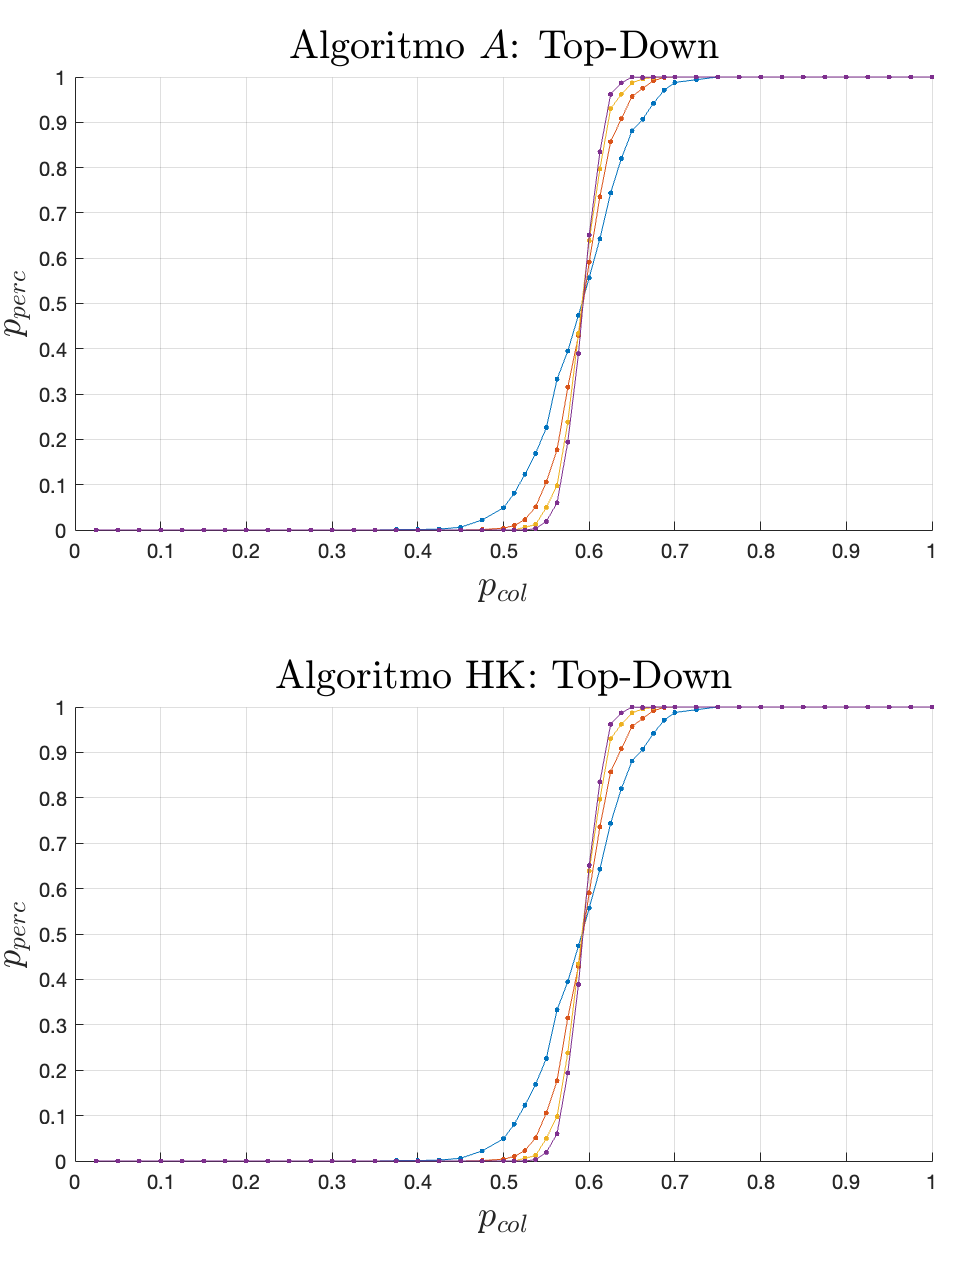
\includegraphics[width=\columnwidth]{compare_threshold_1.png}
    \caption{Confronto tra le frequenze di percolazione top-down ottenute nell'esecuzione
    dei due algoritmi.}
    \label{fig:compare_threshold}
\end{figure}
Risulta interessante eseguire un confronto con la Fig. \ref{fig:threshold} 
relativa al reticolo di taglia infinita: per dimensioni del reticolo più grandi, ci 
si avvicina infatti al suddetto grafico.
Un'altra caratteristica importante da verificare è che le frequenze di 
percolazione top-down registrate coincidano con quelle left-right, nel limite 
dell'errore commesso. Le modalità di svolgimento sono le stesse, con l'aggiunta 
delle misurazioni dell'errore, calcolato come radice quadrata della quantità 
$D_{f_{perc}}$ descritta nell'Eq. \ref{eq:d_f_perc}.
Nel grafico in Fig. \ref{fig:th_errors} viene mostrato un confronto tra i valori 
ottenuti nei due casi con l'algoritmo HK. Ciò che balza all'occhio è la 
superiorità degli errori intorno a $0.6$, valore in cui, tra l'altro, 
si osserva una crescita piuttosto rapida della frequenza di percolazione.
\begin{figure}[ht]
    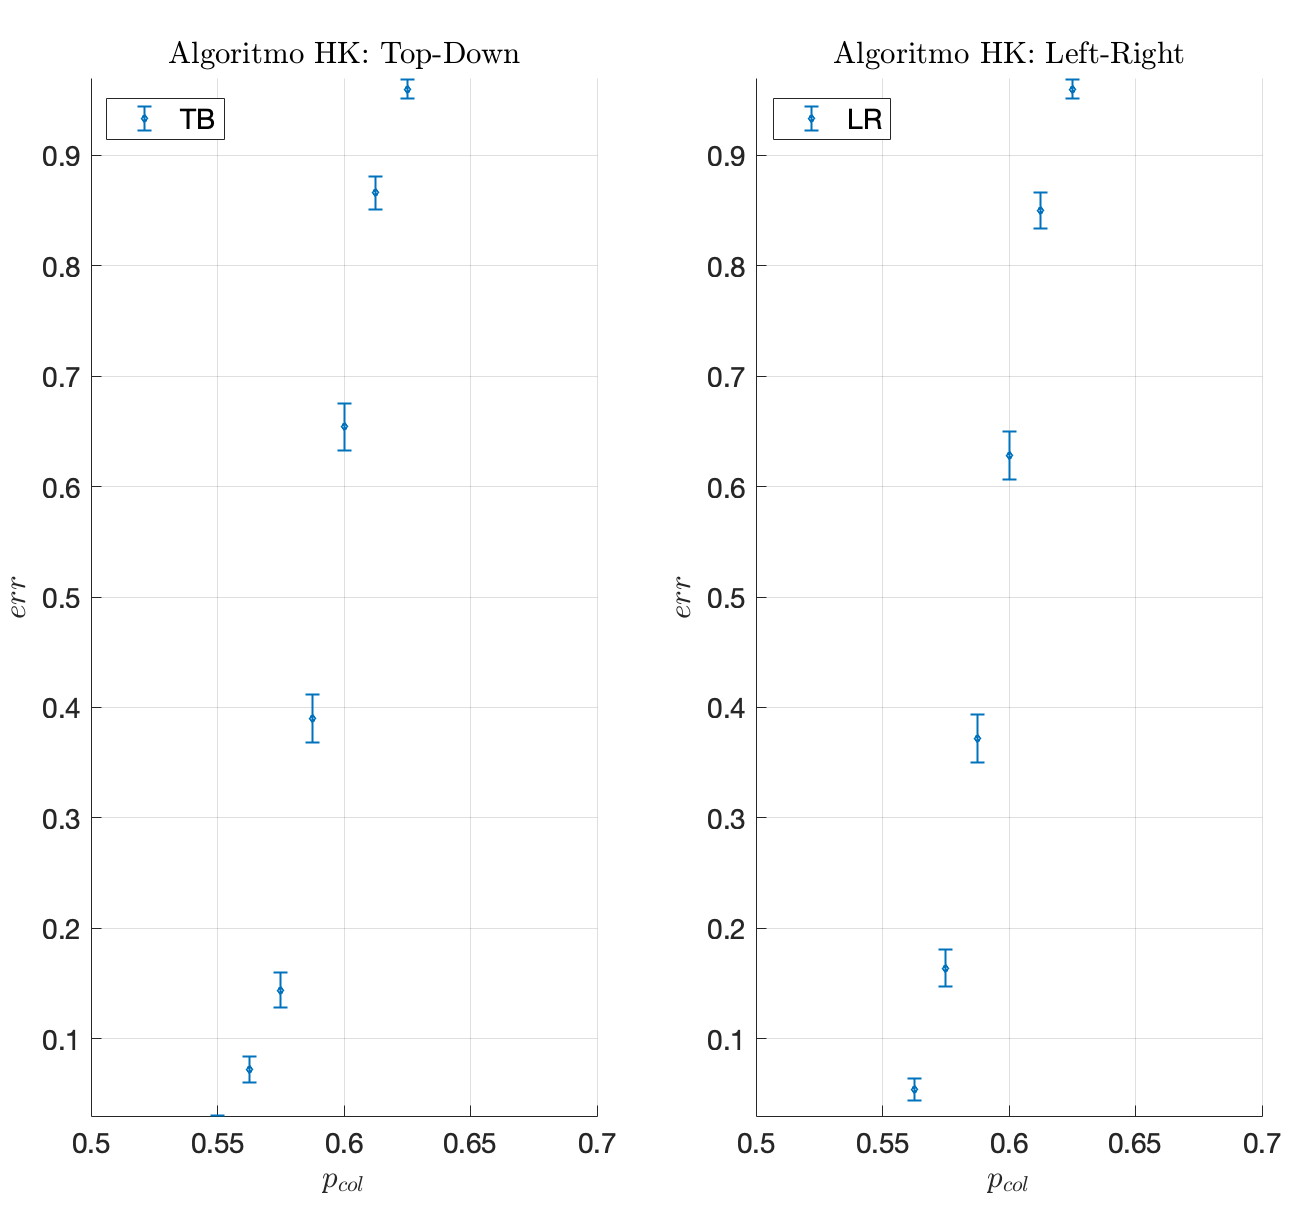
\includegraphics[width=\columnwidth]{errors.png}
    \caption{Confronto tra le frequenze di percolazione top-down e left-right,
    con rispettivi errori.}
    \label{fig:th_errors}
\end{figure}

Inserire porzione del codice.

\subsection*{Calcolo delle osservabili}

\subsection*{Tempi di esecuzione}